%%%%%%%%%%%%%%%%%%%%%%%%%%%%%%%%%%%%%%%%%%%%%%%%%%%%%%%%%%%%%%%%%
%        Contents: Bachelorarbeit, HS Fulda        %
%                          31.08.2022                        %
%---------------------------------------------------------%
%                         Bewertung.tex                     %
%                        by Fangfang Tan                    %
%         fangfang.tan@informatik.hs-fulda.de      %
%%%%%%%%%%%%%%%%%%%%%%%%%%%%%%%%%%%%%%%%%%%%%%%%%%%%%%%%%%%%%%%%%

\chapter{Bewertung der Technologien} \label{EV}

Eines der Ziele dieser Bachelorarbeit ist es, die Vor- und Nachteile von SAP AppGyver, SAP Fiori Elements und SAPUI5 zu identifizieren und herauszufinden, welche Technologie für welche Implementierungsszenarien geeignet ist. In Kapitel 3 und 4 wurden die technische Umsetzung und weitere Funktionen beschrieben. In diesem Kapitel werden nun zwei Bewertungsmatrizen definiert, diese mit Bewertungen gefüllt und anschließend die Bewertungsergebnisse interpretiert und diskutiert.

Die Bewertungsmatrizen beziehen sich zum einen auf die Bewertung der Funktionen des jeweiligen Tools, sowie die Möglichkeit zur Abbildung der definierten Anforderungen. Eine zweite Matrix wird dann für die Entwickler-Perspektive angefertigt.

\section{Bewertungsmatrixen definieren}
Die Bewertungsmatrizen besitzen die Form einer Tabelle \cite{wi:ma} und jeweils einen Tabellenkopf mit den Spaltenbezeichnungen, eine Tabellenvorspalte mit der Beschreibung der Funktionen und die Bewertung als eigentlichen Tabelleninhalt. Der Tabelleninhalt zeigt so die Zusammenhänge zwischen den Zeilen und Spalten. \cite{wi:ta} 

\subsection{Bewertungsmatrix zur Implementierung der Funktionalität}
In Kapitel 3 und 4 wurde die technische Umsetzung der Anforderungen oder eventuell vorhandene Umsetzungsansätze im Detail beschrieben. Dabei lassen sich diese grundsätzlich in zwei Bereiche aufteilen: Backend- und Frontend-Funktionalität. 
Die Backend-Funktionen umfassen:
\begin{itemize}[noitemsep]
\item Möglichkeiten zur Datenmodellierung.
\item Möglichkeiten zur Datenerstellung, -speicherung, -bearbeitung und löschung.
\item Möglichkeiten zur zentralen Datenbereitstellung.
\end{itemize}
Es wurde bereits darauf hingewiesen, dass nicht alle Tools über diese Art von Backend-Funktionalitäten verfügen.
In Kapitel 3 und Kapitel 4 wurden weiterhin diverse Frontend-Funktionen implementiert und untersucht. Tabelle 5.1 zeigt die volle Bewertungsmatrix der Funktionen.

\begin{table}[htbp]\small
    \centering
    \setlength{\leftmargini}{0.4cm}
    \begin{tabular}{|>{\columncolor{mygrey2}}  p{4cm}  | l | l | l |}
        \hline
        \rowcolor{mygrey2} \diagbox{Funktionen}{Tools} & Fiori Elements mit CAP & AppGyver & SAPUI5  \\
        \hline
        Datenmodellierung & & &  \\
        \hline
        \makecell[l]{Datenerstellung, \\ -speicherung, \\ -bearbeitung \\ und -löschung} &  &  &  \\
        \hline
        Servicebereitstellung & & &  \\
        \hline
        \makecell[l]{Listansicht zur Anzeige \\ aller Produkte} & & & \\
        \hline
        \makecell[l]{Einzelansicht für ein \\ Produkt} & & &  \\
        \hline
        \makecell[l]{Maske zum Pflegen eines \\ einzelnen Produkts} & & &  \\
        \hline
        \makecell[l]{Integration von \\Suchfiltern} &  &  &  \\
        \hline
        \makecell[l]{Integration von \\Paginierung} &  &  &  \\
        \hline
        \makecell[l]{Integration von Bild und \\ PDF-Dateien} & & &  \\
        \hline
        \makecell[l]{Integration einer Barcode \\ Scanner Funktionen} & & & \\
        \hline
        \makecell[l]{Nutzung mobiler \\ Funktionen} & & &  \\
        \hline
        \makecell[l]{Deployment für \\ unterschiedliche Endgeräte} & & & \\
        \hline
        \makecell[l]{Freie \\ Gestaltungsmöglichkeiten} & & &  \\
        \hline
    \end{tabular}
  \caption{Bewertungsmatrix zur Implementierung der Funktionalität} 
\end{table}

Der Inhalt der Matrix wird mit Punktwerten belegt. Die Bewertungsmatrix umfasst zwei grundsätzliche Bewertungskriterien: die Umsetzbarkeit der zu bewertenden Funktionalitäten und den Implementierungsaufwand. Die Erfüllung der Kriterien wird auf einer Skala von 0 bis 3 eingestuft. Ein Wert von 0 bedeutet, dass die bewertete Funktion nicht umgesetzt werden kann. Der Aufwand wird im Rahmen dieser Bachelorarbeit wie folgt definiert: Der Aufwand wird gleichgesetzt mit der zeitlichen Dauer der Umsetzung, gemessen in Personentagen. Die Dauer umfasst dabei lediglich die reine technische Implementierungszeit und keine weiteren Aktivitäten, wie Konzeption, Testen oder Dokumentation. Die zeitliche Bewertung folgt dabei dem Wissenstand der Autorin in der jeweiligen Rolle:

\begin{itemize}[noitemsep]
\item Citizen Developer: SAP AppGyver und SAP Fiori Elements.
\item Pro Developer: SAPUI5.
\end{itemize}

Ein Wert von 1 bedeutet, dass die Funktion zwar implementiert werden kann, aber nur mit einem hohen Aufwand, also einer Umsetzungsdauer von mehr als 1 Personentag. Ein Wert von 2 bedeutet, dass die Umsetzung zwischen 0,5 bis 1 Personentage in Anspruch nimmt. Ein Wert von 3 bedeutet, dass die Funktion schnell umgesetzt werden kann, in wenigen Minuten bis zu einem halben Personentag.

\begin{table}[htbp]
    \centering
    \begin{tabular}{| c |}
        \hline
        \rowcolor{mygrey2} Erfüllungskriterien: 0 bis 3  \\
        \hline
        \makecell[l]{0 = nicht umsetzbar \\ 1 = mehr als 1 PT \\ 2 = 0,5 bis 1 PT \\ 3 = weniger als 0,5 PT}  \\
        \hline
    \end{tabular}
 \caption{Erfüllung Kriterien der Bewertungsmatrix} 
\end{table}


 \pagebreak
\subsection{Bewertungsmatrix für die Entwicklerperspektive}
Für die Entwicklerperspektive wird eine Matrix zur Bewertung der Entwicklungsumgebungen und Entwicklungstools für die drei Technologien definiert. Folgende Tabelle liefert eine Auflistung aller Bewertungskriterien: 
\begin{table}[htbp]\small
    \centering
    \setlength{\leftmargini}{0.4cm}
    \begin{tabular}{|>{\columncolor{mygrey2}}  p{4cm}  | l | l | l |}
        \hline
        \rowcolor{mygrey2} \diagbox{\makecell[l]{Entwickle-\\perspektive}}{Tools} & Fiori Elements mit CAP & AppGyver & SAPUI5  \\
        \hline
        \makecell[l]{Notwendiges technisches \\ Verständnis} & & &  \\
        \hline
        \makecell[l]{Bedienbarkeit der \\ Entwicklungsumgebung} &  &  &  \\
        \hline
        \makecell[l]{Vollständigkeit der \\ Funktionen der \\ Entwicklungsumgebung} & & &  \\
        \hline
        \makecell[l]{Spezialisierung der \\ Entwicklungsumgebung} & & & \\
        \hline
        \makecell[l]{Einrichtungsaufwand der \\ Entwicklungsumgebung} & & &  \\
        \hline
        \makecell[l]{Unabhängigkeit der \\ Entwicklungsumgebung \\von Betriebssystem} & & &  \\
        \hline
        \makecell[l]{Stabilität der \\ Entwicklungsumgebung} &  &  &  \\
        \hline
        \makecell[l]{Dokumentation für \\ Programmierer} & & &  \\
        \hline
        Debugger & & & \\
        \hline
        Versionsverwaltung & & &  \\
        \hline
    \end{tabular}
  \caption{Bewertungsmatrix aus der Entwickler-Perspektive} 
\end{table}

Der Inhalt der Matrix wird auch hier mit Punktwerten belegt, wobei jede Tabellenvorspalte eigene Bewertungskriterien umfasst. Die Erfüllung der Kriterien wird auf einer Skala von 1 (grundsätzlich negativ) bis 3 (grundsätzlich positiv) eingestuft. Die Erfüllungskriterien werden in Tabelle 5.4 detailliert vorgestellt.

\begin{table}[htbp]\small
    \centering
    \setlength{\leftmargini}{0.4cm}
    \begin{tabular}{|>{\columncolor{mygrey2}}  p{4cm}  | p{3cm} | p{3cm} | p{3cm} |}
        \hline
        \rowcolor{mygrey2} \diagbox{\makecell[l]{Entwickle-\\perspektive}}{\makecell[r]{Erfüllungs-\\kriterien}} & 1 & 2 & 3  \\
        \hline
        \makecell[l]{Notwendiges technisches \\ Verständnis} & Programmier-ausbildung notwendig  & Grundlegende IT-Prinzipien notwendig & Kein IT-Verständnis notwendig  \\
        \hline
        \makecell[l]{Bedienbarkeit der \\ Entwicklungsumgebung} & Komplex und nur mit mehrfacher Anleitung/nach Schulung bedienbar  &  Komplexer, aber nach erstmaliger Nutzung verständlich & Einfach und selbsterklärend   \\
        \hline
        \makecell[l]{Vollständigkeit der \\ Funktionen der \\ Entwicklungsumgebung} & Wichtige Funktionen fehlen & Funktionen fehlen, können aber über Erweiterungen installiert werden & Alle notwendigen Funktionen integriert \\
        \hline
        \makecell[l]{Spezialisierung der \\ Entwicklungsumgebung} & exklusiv und nicht für andere Dinge nutzbar & Unterstützung weiterer Programmiersprachen und Anwendungstypen & Offen und Unterstützung vieler Anwendungsfälle  \\
        \hline
        \makecell[l]{Einrichtungsaufwand der \\ Entwicklungsumgebung} & Hoch (Manuell, mehrstufig, Dauer > 1 Stunde) & Mittel (Manuell, Konfiguration notwendig, Dauer > 10 Minuten < 1 Stunde) & Niedrig (Automatisch, nur wenig Konfiguration, Dauer < 10 Minuten) \\
        \hline
        \makecell[l]{Plattformunabhängigkeit  \\ der Entwicklungsumgebung} & Spezifisch & Teilweise abhängig & Systemunabhängig \\
        \hline
        \makecell[l]{Stabilität der \\ Entwicklungsumgebung} & Instabil inklusive Datenverlust  & Gelegentliche Instabilität &  Stabil \\
        \hline
        \makecell[l]{Dokumentation für \\ Programmierer} & Nicht vorhanden & Unvollständig & Vollständig \\
        \hline
        Debugger & Nicht vorhanden & Komplexe Nutzung & Einfache Nutzung \\
        \hline
        Versionsverwaltung & Nicht integriert & Integrierbar & Integriert  \\
        \hline
    \end{tabular}
  \caption{Erfüllungskriterien aus der Entwickler-Perspektive} 
\end{table}

\section{Durchführung der Bewertung}

\subsection{Bewertung zur Implementierung der Funktionalität}
An dieser Stelle sollte darauf hingewiesen werden, dass die Bewertung für den Aufwand subjektiv ist und aus der Sicht anderer, insbesondere erfahrener Entwickler, abweichen kann. 
Die Backend-Funktionalitäten wie Datenmodellierung, die Unterstützung von CRUD-Funktionalitäten, sowie die Servicebereitstellung mit Fiori Elements in Verbindung mit CAP wurden bereits in Kapitel 3.1.2 vorgestellt. Durch die sehr gute Integration in die Entwicklungsumgebung, können dort alle Dinge mit geringem Aufwand über Eingabemasken realisiert werden. 
SAP AppGyver bietet ebenfalls Funktionalitäten an, Datenstrukturen anzulegen und Daten zu speichern. Zur Datenmodellierung gibt es ein spezielles Data-Tool. (siehe Abbildung 5.1).

\begin{figure}[!htbp]
 \centering
 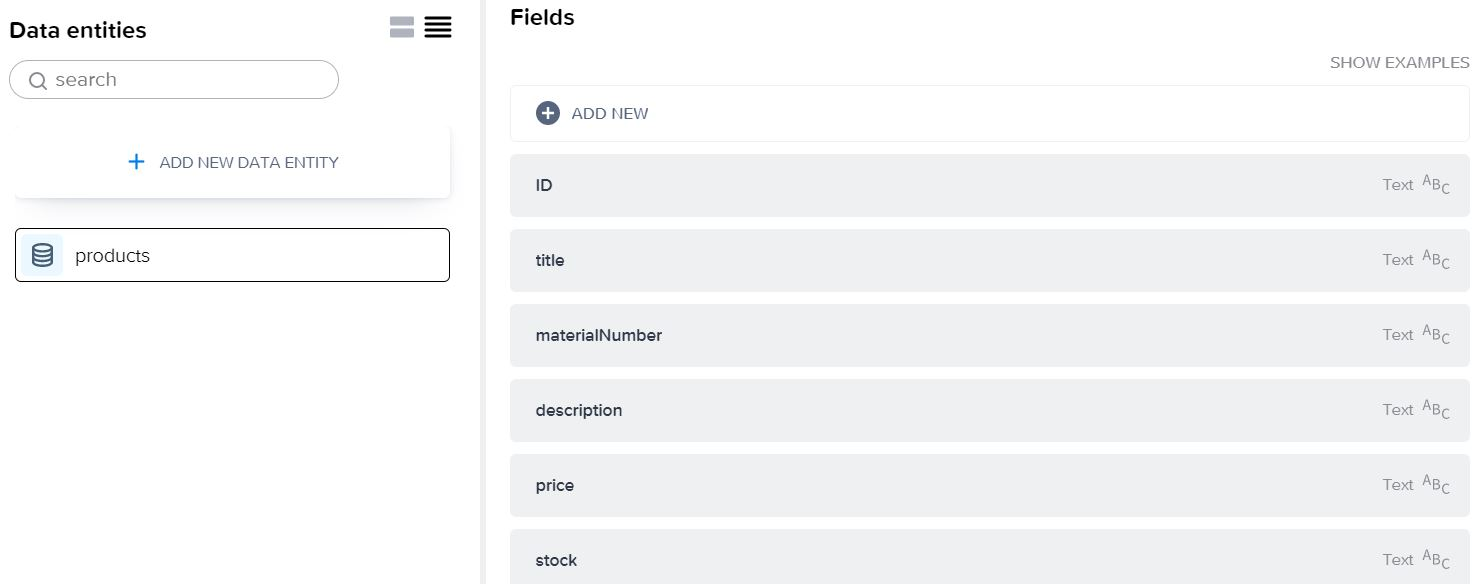
\includegraphics[width=0.6\textwidth]{Bilder/appgyver/5_1_Daten moddeliereung.jpg}
 \caption{Daten Modellierung in AppGyver}
\end{figure}

Unter „Capabilities“ sieht man, dass die Standard-Operationen auf die Daten direkt in eine AppGyver-Anwendung integriert werden (Abbildung 5.2). Grundsätzlich werden die Daten jedoch direkt und nur in der Anwendung gespeichert. Eine zentrale Bereitstellung als OData-Service ist mit AppGyver nicht möglich.

\begin{figure}[!htbp]
 \centering
 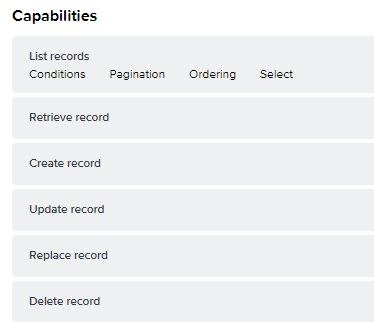
\includegraphics[width=0.4\textwidth]{Bilder/appgyver/5_2_Capabilities.jpg}
 \caption{Daten-Capabilities in AppGyver}
\end{figure}

SAPUI5 unterstützt als reine Frontend-Technologie nicht die Erstellung von Backend-Datenstrukturen und OData-Services. Für die Integration eines Backend-Layers müsste analog zu SAP Fiori Elements das Cloud Application Programming-Model (oder eine andere Backend-Technologie) hinzugenommen werden. Da es hier jedoch keine einfache Integration in die Entwicklungsumgebung (VS-Code) gibt, müsste der Backend-Part manuell implementiert werden. Dies ist zwar in Sachen Implementierungsaufwand überschaubar (Quelltext 5.1 zeigt die Definition der Datenstrukturen, Quelltext 5.2 das Exponieren als OData-Service), allerdings muss der Entwickler neben dem SAPUI5- auch das CAP-Programmiermodell verstehen.

\begin{lstlisting}[emph={using, entity, Products, title, description, materialNumber, price, stock, String},  caption=Datenmodellierung in der \texttt{model.cds}]
using { cuid } from '@sap/cds/common';
namespace db;
entity Products: cuid{
    title: String(1000);
    description: String(1000);
    materialNumber: Integer;
    price: String(100);
    stock: String(100);
}
\end{lstlisting}
\begin{lstlisting}[emph={using, entity, db, Products},  caption=Service Bereitstellung in der \texttt{public\_service.cds}]
using db from '../db/model';
service PublicService{
    entity Products as projection on db.Products;
}
\end{lstlisting}

Tabelle 5.5 stellt die Bewertung des Implementierungsaufwands zur Datemodellierung, Datenerstellung, -speicherung, -bearbeitung und -löschung, sowie die Servicebereitstellung dar.

\begin{table}[htbp]\small
    \centering
    \setlength{\leftmargini}{0.4cm}
    \begin{tabular}{|>{\columncolor{mygrey2}}  p{3.9cm}  | l | l | l |}
        \hline
        \rowcolor{mygrey2} \diagbox{Funktionen}{Tools} & Fiori Elements mit CAP & AppGyver & SAPUI5  \\
        \hline
        Datenmodellierung & 3 & 3 & 0 \\
        \hline
        \makecell[l]{Datenerstellung, \\ -speicherung, \\ -bearbeitung \\ und -löschung} & 3 & 3 & 0  \\
        \hline
        Servicebereitstellung & 3 & 0 & 0  \\
        \hline
    \end{tabular}
  \caption{Bewertung der Backend-Funktionen} 
\end{table}

In Kapitel 3 wurde eine Anwendung implementiert, die eine Listenansicht, eine Einzelansicht und eine Maske zur Pflege eines einzelnen Produkts enthält. Tabelle 5.6 zeigt die Bewertungsergebnisse des Implementierungsaufwands dieser Funktionalitäten:

\begin{table}[htbp]\small
    \centering
    \setlength{\leftmargini}{0.4cm}
    \begin{tabular}{|>{\columncolor{mygrey2}}  p{3.9cm}  | l | l | l |}
         \hline
        \rowcolor{mygrey2} \diagbox{Funktionen}{Tools} & Fiori Elements mit CAP & AppGyver & SAPUI5  \\
        \hline
        \makecell[l]{Listansicht zur Anzeige \\ aller Produkte} & 3 & 3 & 2\\
        \hline
        \makecell[l]{Einzelansicht für ein \\ Produkt} & 3 & 2 & 2\\
        \hline
        \makecell[l]{Maske zum Pflegen eines \\ einzelnen Produkts} & 3 & 2 & 1 \\
        \hline
    \end{tabular}
  \caption{Bewertung der Grundlistenfunktionen} 
\end{table}

Hier lässt sich herausstellen, dass Fiori Elements diese Sichten in Form eines Floorplans direkt bereitstellt und der Implementierungsaufwand entsprechend gering ist. In AppGyver und SAPUI5 müssen diese Dinge manuell nachgebaut werden, was einen größeren Aufwand bedeutet. AppGyver ist durch die Möglicheit zum Drag\&Drop hier jedoch deutlich schneller.
In Kapitel 4 wurden weitere Funktionen untersucht, um Fiori Elements, AppGyver und SAPUI5 eingehender zu betrachten. Der geschätzte Implementierungsaufwand und Umsetzbarkeit dieser Funktionen werden in Tabelle 5.7 dargestellt. 

\begin{table}[!htbp]\small
    \centering
    \setlength{\leftmargini}{0.4cm}
    \begin{tabular}{|>{\columncolor{mygrey2}}  p{4cm}  | l | l | l |}
        \hline
        \rowcolor{mygrey2} \diagbox{Funktionen}{Tools} & Fiori Elements mit CAP & AppGyver & SAPUI5  \\
        \hline
        \makecell[l]{Integration von \\ Suchfiltern} & 3 & 3 & 2 \\
        \hline
        \makecell[l]{Integration von \\ Paginierung} & 3 & 1 & 3  \\
        \hline
        \makecell[l]{Integration von Bild und \\ PDF-Dateien} & 1 & 3 & 3 \\
        \hline
        \makecell[l]{Integration einer Barcode \\ Scanner Funktionen} & 1 & 3 & 1\\
        \hline
        \makecell[l]{Nutzung mobiler \\ Funktionen} & 1 & 2 & 1  \\
        \hline
        \makecell[l]{Deployment für \\ unterschiedliche Endgeräte} & 1 & 3 & 1 \\
        \hline
        \makecell[l]{Freie \\ Gestaltungsmöglichkeiten} & 1 & 3 & 3  \\
        \hline
    \end{tabular}
  \caption{Bewertung der weiteren Funktionen} 
\end{table}

Suchfilter und Paginierung lassen sich sehr einfach in Fiori Elements umsetzen, da sie Teil des Floorplans sind. Alle weiteren Dinge sind jedoch mit hohem Aufwand umzusetzen, da sie aufwändig über Erweiterungen hinzuprogrammiert werden müssten. In AppGyver lassen sich alle weiteren Funktionen umsetzen, die meisten mit geringem Aufwand. Lediglich die Paginierung erfordert eine komplexere Umsetzung. Mit SAPUI5 können ebenfalls alle Funktionen abgebildet werden. Allerdings ist hier der Implementierungsaufwand stets höher durch das notwendige Coding.

\subsection{Bewertung von der Entwicklerperspektive}
Wie auch die Bewertung der Funktionen, ist die Beurteilung der Entwicklerperspektive mit subjektiven Eindrücken durch die die Erfahrung der Autorin geprägt. Auch hier wurden die Grundkenntnisse während der Anfertigung der Thesis erarbeitet und können von den Ergebnissen erfahrener Anwender abweichen. 
\begin{table}[!htbp]\small
    \centering
    \setlength{\leftmargini}{0.4cm}
    \begin{tabular}{|>{\columncolor{mygrey2}}  p{4cm}  | l | l | l |}
        \hline
        \rowcolor{mygrey2} \diagbox{\makecell[l]{Entwickle-\\perspektive}}{Tools} & Fiori Elements mit CAP & AppGyver & SAPUI5  \\
        \hline
        \makecell[l]{Notwendiges technisches \\ Verständnis} & 3 & 2 & 1 \\
        \hline
        \makecell[l]{Bedienbarkeit der \\ Entwicklungsumgebung} & 3 & 2 & 1  \\
        \hline
        \makecell[l]{Vollständigkeit der \\ Funktionen der \\ Entwicklungsumgebung} & 2 & 3 & 3  \\
        \hline
        \makecell[l]{Spezialisierung der \\ Entwicklungsumgebung} & 2 & 1 & 3 \\
        \hline
        \makecell[l]{Einrichtungsaufwand der \\ Entwicklungsumgebung} & 3 & 3 & 1 \\
        \hline
        \makecell[l]{Unabhängigkeit der \\ Entwicklungsumgebung \\von Betriebssystem} & 3 & 3 & 2 \\
        \hline
        \makecell[l]{Stabilität der \\ Entwicklungsumgebung} &  2 & 3 & 3 \\
        \hline
        \makecell[l]{Dokumentation für \\ Programmierer} & 2 & 2 & 1 \\
        \hline
        Debugger & 3 & 1 & 3 \\
        \hline
        Versionsverwaltung & 3 & 2 & 3 \\
        \hline
    \end{tabular}
  \caption{Bewertungsmatrix aus der Entwicklerperspektive} 
\end{table}
Tabelle 5.8 zeigt die Bewertungsergebnisse aus der Entwicklerperspektive. Begründete Erklärungen finden sich nachfolgend.

Das notwendige technische Verständnis für die Umsetzung von Applikationen ist nicht einfach zu bewerten. Tatsächlich verlangte die Umsetzung von Fiori Elements in BAS lediglich das Ausfüllen von Formular-Dialogen und ist per Definition No-Code. Möchte man jedoch an irgendeiner Stelle vom Standardverhalten abweichen, dann ist das tiefgreifende Verständnis von JavaScript, SAPUI5 und Co notwendig. Da die Anforderungen jedoch mit der Standardfunktionalität umgestzt werden konnten, ist die Bewertung hier entsprechend gut (Bewertung 3). SAP AppGyver verlangt das grundlegende Verständnis von Kernprinzipien in der IT, wie technische Schnittstellen (REST, OData), UI-Events, (komplexe) Formeln, Data-Binding und Daten-, bzw. Logikflüsse. Ein Programmierer mit geringen IT-Kenntnissen wird hier bei der Erstellung deutlich überfordert sein. Für SAPUI5 ist definitiv eine Programmierausbildung notwendig und wird deswegen mit 1 bewertet.

Bei BAS handelt es sich zwar eine flexible Entwicklungsumgebung, die in vielen Bereichen ähnlich zu bedienen ist wie VS-Code, die Dialoge für die Fiori Elements-Entwicklung sind jedoch gezielt einfach gehalten und verstecken die Komplexität. Composer Pro für SAP AppGyver ist eine spezialisierte Umgebung, die versucht, die Funktionaltäten möglichst einfach abzubilden. Durch die Fülle an Funktionen sind manche Dinge jedoch komplex zu bedienen (Bewertung 2). Bei VS-Code handelt es sich um ein sehr mächtiges Werkzeug, das zwar Wert auf eine einfache Bedienung legt, viele Funktionen aufgrund der Komplexität jedoch erst nachgeschlagen werden müssen (Bewertung 1).

Der Einrichtungsaufwand von BAS und AppGyver Composer Pro (Enterprise-Version) ist mit wenigen Mausklicks durchführbar, da es sich hierbei um Software-as-a-Service-Umgebungen handelt. Beide müssen nur vom SAP BTP Service Marketplace zum eigenen SAP BTP-Subaccount hinzugefügt werden. Danach stehen sie für die Entwicklung bereit. Der Einrichtungsaufwand für die AppGyver Community-Version ist sogar noch geringer, da man sich lediglich bei AppGyver Composer Pro registrieren und anmelden muss. Der Einrichtungsaufwand in VS-Code für die Entwicklung der SAPUI5-Anwendung ist deutlich höher, da hier die Umgebung lokal auf dem Rechner installiert wird und noch weitere Tools, Generatoren und Extensions heruntergeladen und installiert werden müssen. Deswegen wird auch hier die geringste Punktzahl vergeben.

Grundsätzlich sind alle drei Entwicklungsumgebungen unabhängig vom Betriebssystem. Bei VS-Code müssen jedoch alle Dinge lokal installiert werden, mitunter auch betriebssystemspezifisch. Im Kontext der Arbeit gab es an wenigen Stellen Unterschiede zwischen Windows und MacOS, weswegen VS-Code (SAPUI5) mit 2 bewertet wurde.

Ein Nachteil von web-basierten-Umgebungen ist die Tatsache, dass man abhängig von der Verfügbarkeit des Anbieters ist. Während des Anfertigens der Thesis stürzte das BAS zweimal ab und war danach für mehrere Stunden nicht verfügbar. Deswegen wird BAS (Fiori Elements) hier nur mit 2 Punkten bewertet. Composer Pro und VS-Code liefen komplett stabil.

Ressourcen für die Unterstützung von Entwicklern sind Dokumentationen, Online-Tutorials, Online-Foren, Bücher und E-Books. Eine Stärke von SAPUI5 ist die umfangreiche Dokumentation mit Control- und Code-Beispielen und einer vollständigen API-Dokumentation. Deswegen erhält SAPUI5 hier die volle Punktzahl. Für AppGyver und Fiori Elements sind deutlich weniger Ressourcen verfügbar, weswegen sie hier schlechter bewertet werden.

Das Debugging ist während der Entwicklung einer Anwendung sehr wichtig, um die Logik zu überprüfen. Zum Debuggen der UI5-Webanwendung können die Browser-Tools (Google DevTools oder Microsoft Edge DevTools) verwendet werden, die sehr bedienungsfreundlich sind. Mit dem Debugger von AppGyver Community Edition kann der Entwickler die Mobile App zwar diagnostizieren, aber die Bedienung des Debuggers ist sehr kompliziert. Außerdem ist die Verbindung zwischen Mobile App und AppGyver Debugger nicht immer stabil. Der Debugger ist derzeit für die SAP Enterprise-Edition sogar gar nicht verfügbar, weswegen die Bewertung hier bei 1 Punkt liegt. Die Entwicklung mit Fiori Elements erfordert kein Debugging.

Obwohl es sich bei der Erstellung der Fiori-Anwendung um No-Code handelt, wird im Hintergrund automatisch Quellcode generiert. Zur Verwaltung des Quellcodes in Fiori Elements und SAPUI5 gibt es Tools wie Git. Basierend auf dem Quellcode kann der Entwickler mit git mehrere Code-Linien (Branches) gleichzeitig, sowie Entwicklungs-Snapshots (Commit) verwalten. In BAS und VS-Code ist git nativ integriert und dementsprechend wird hier die volle Punktzahl vergeben. Das “Release Management” in der AppGyver Enterprise-Edition bietet eine einfache Snapshot und Rollback Funktion für die Versionsverwaltung [Moh22], aber keine vollumfängliche Funktionalität wie git. So kann man beispielsweise nur eine einzelne Release-Linie verwalten. In der AppGyver Community-Edition ist das „Release Management“ gar nicht verfügbar. 

\section{Interpretation und Diskussion}
Zwar wurden die einzelnen Funktionen und Aspekte der Entwicklungsumgebungen im Vorherigen punktuell bewertet, es wird jedoch an dieser Stelle keine Summe und damit Rangfolge gebildet, sondern jedes Tool für sich einzeln analysiert und im Hinblick auf die Fragestellungen der Arbeit bewertet:
\begin{itemize}[noitemsep]
\item Welche Vor- und Nachteile dieser drei Technologien lassen sich durch die exemplarische Umsetzung herausstellen? 
\item Welche Technologie eignet sich in Zukunft für welche Umsetzungsszenarien?
\end{itemize}

Zur besseren visuellen Interpretation kommen Netzdiagramme zum Einsatz. Bei diesen werden die einzelnen Kategorien in Form eines Kreises angeordnet und die Werte auf der Basis von 0 bis 3 gezeichnet und verbunden.

\subsection{SAP Fiori Elements in Verbindung mit Business Application Studio}
Das Netz-Diagramm zur Umsetzung der Anforderungen mit Fiori Elements zeigt sehr gut, dass sich die unterstützten Standardfunktionalitäten sehr gut und schnell umsetzen lassen. Deutlich schneller als mit den beiden anderen betrachteten Werkzeugen. Sobald man jedoch von der Standard-Funktionalität der Floorplans abweicht, wird die Umsetzung aufwendig.
So wird dann auch aus dem No-Code-Ansatz direkt ein Pro-Code, der eine komplexere Programmierung erfordert. Dies stellt auch eine Frage an die potenzielle Zielgruppe für Fiori Elements: Zwar kann ein geschulter Citizen Developer schnell Ergebnisse erzielen, er muss jedoch bei Erweiterungen entweder auch ein Pro-Developer sein oder auf einen solchen zurückgreifen.
\begin{figure}[!htbp]
 \centering
 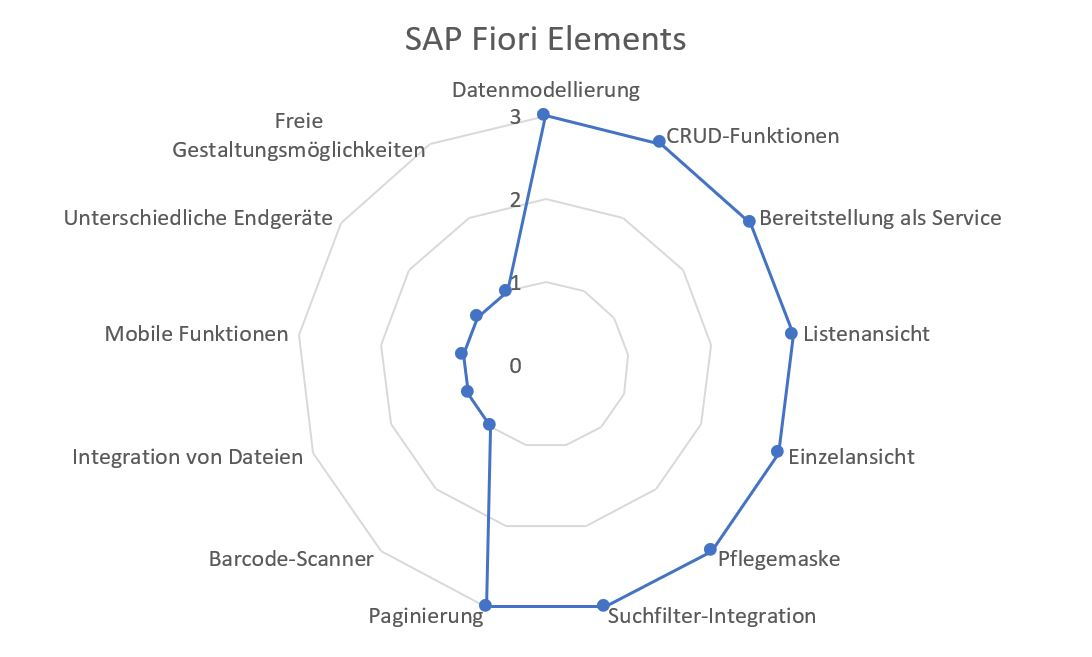
\includegraphics[width=0.7\textwidth]{Bilder/bewertung/ND_fiori.jpg}
 \caption{Bewertung von Umsetzung der Anforderungen mit Fiori Elements}
\end{figure}

\pagebreak
Die Fragestellung stellt sich ebenfalls bei der Betrachtung des Business Application Studios. Hierbei handelt es sich um eine volle Entwicklungsumgebung, die jedoch spezielle No-Code-Sichten für Fiori Elements und CAP bereitstellt. Der Sprung von No-Code zu Pro-Code kann somit innerhalb von wenigen Mausklicks erfolgen. No-Code- und Pro-Code-Entwickler müssten deswegen in der gleichen Entwicklungsumgebung arbeiten. Dies legt nahe, dass die Zielgruppe eigentlich Pro-Code-Entwickler sind, die für Standard-Anwendungen mit Fiori Elements sehr schnell Ergebnisse erzielen und diese bei Bedarf erweitern können.

\begin{figure}[!htbp]
 \centering
 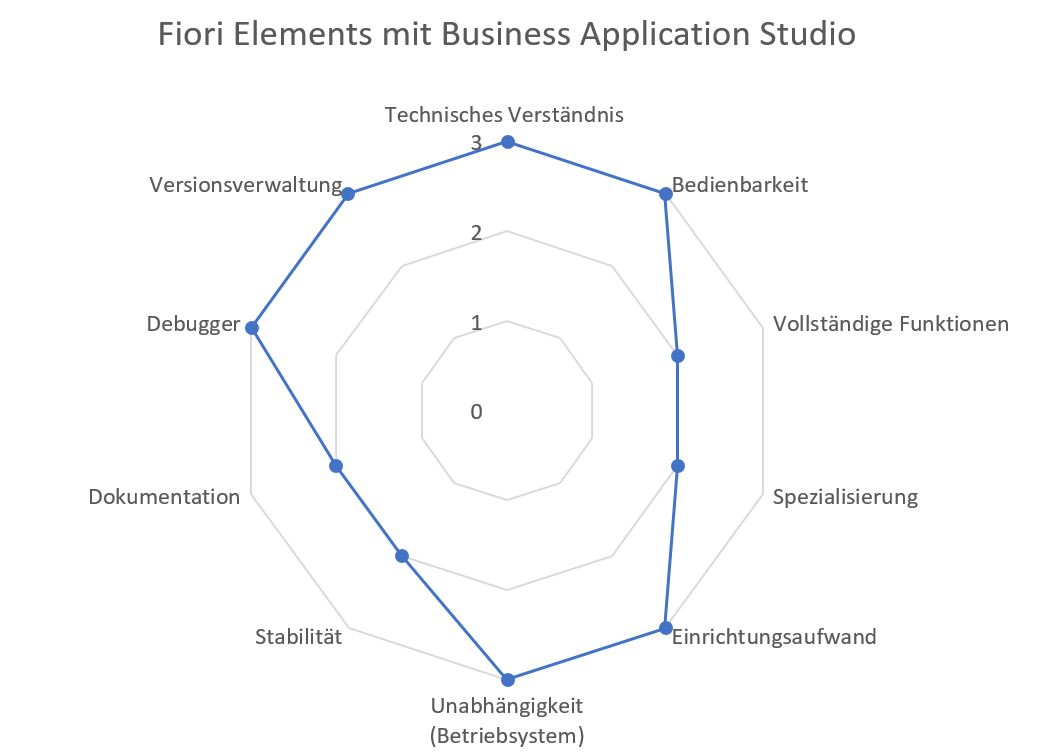
\includegraphics[width=0.7\textwidth]{Bilder/bewertung/ND_fiori_BSP.jpg}
 \caption{Bewertung von Fiori Elements mit BAS}
\end{figure}

Die Vor- und Nachteile von SAP Fiori Elements in Verbindung mit Business Application Studio lassen sich wie folgt zusammenfassen:
\begin{table}[!htbp]
    \centering
     \setlength{\leftmargini}{0.4cm}
    \begin{tabular}{| m{6cm} | m{6cm} |}
        \hline
        \rowcolor{mygrey2} \makecell[c] {Vorteile} & \makecell[c] {Nachteile} \\
        \hline
         \begin{itemize} 
            \item Sehr schnelle Umsetzung von Backend- und Frontend-Apps, basierend auf fest definierten Floorplans
            \item Komfortable Entwicklungsumgebung 
            \item Integration von fortschrittlichen Entwicker-Tools (git)
        \end{itemize} & 
        \begin{itemize} 
            \item Großer Aufwand für Funktionalitäten außerhalb des Floorplans
            \item Keine Freiheitsgrade bei der Gestaltung der Apps
            \item Probleme mit Stabilität von BAS
            \item Wenig Dokumentation für Entwickler
        \end{itemize} \\
        \hline
      \end{tabular}
  \caption{Vor- und Nachteile von SAP Fiori Elements in Verbindung mit BAS} 
\end{table}

Basierend auf den Vor- und Nachteilen, sowie den diskutierten Details, lassen sich folgende Umsetzungsszenarien ableiten:
\begin{itemize} 
  \item Einfache Standardanwendungen zur Darstellung von Daten in Listen oder einfache CRUD-Anwendungen mit fest vorgegebenem Design in Teams von No-Code-Entwicklern
  \item Standardanwendungen mit sehr geringer funktioneller Abweichung, die von Pro-Entwicklern hinzugefügt werden müssen in gemischten Teams oder in einem Team aus Pro-Code-Entwicklern
\end{itemize}

\subsection{SAP AppGyver in Verbindung mit Composer Pro}
Das Netzdiagramm zur Umsetzung der Anforderungen mit AppGyver zeigt, dass fast alle der untersuchten Funktionalitäten mit AppGyver umgesetzt werden können und die meisten Funktionen einen sehr geringen Aufwand erfordern. Lediglich die Bereitstellung der Daten als zentraler Service ist nicht möglich. 

Im Vergleich zu Fiori Elements dauert die Umsetzung länger und erfordert an diversen Stellen manuellen Low-Code-Entwicklungsaufwand, da die Funktionalitäten nicht per Default bereitstehen. Durch die einfache Bedienung ist die Umsetzung jedoch mit geringem oder mittlerem Zeitaufwand durchzuführen. Und die Vorteile gegenüber Fiori Elements sind auch klar zu benennen: Zusätzliche Funktionen können von der gleichen Entwickler-Gruppe (Low-Code Developer) hinzugefügt werden.

Im Vergleich zu SAPUI5 kann gesagt werden, dass sich beide in vielen Konzepten wie Data Binding, View Controls/Components oder Events ähnlich sind. Die Umsetzung in AppGyver ist aber im Allgemeinen schneller durchzuführen, die die App über spezialisierte Dialoge visuell umgesetzt werden kann. Ein interessanter Aspekt an den gemeinsamen Konzepten ist, dass ein Citizen Developer damit auch ein grundlegendes Verständnis der Konzepte von SAPUI5 besitzt und dies einen potentiellen Entwicklungspfad aufweist.

\begin{figure}[!htbp]
 \centering
 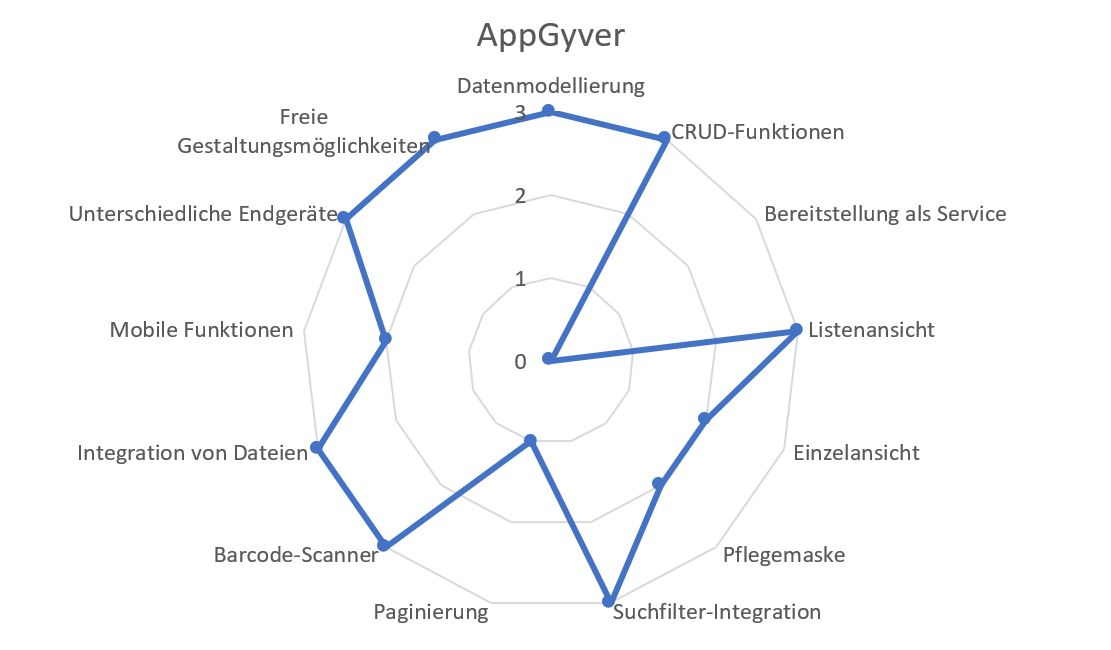
\includegraphics[width=0.7\textwidth]{Bilder/bewertung/ND_AppGyver.jpg}
 \caption{Bewertung von Umsetzung der Anforderungen in AppGyver}
\end{figure}

In Sachen Entwicklungsumgebung ist Composer Pro eine spezialisierte LCNC-Entwicklungsumgebung für AppGyver, die alle notwendigen Funktionen in einer Oberfläche bündelt. 
\begin{figure}[!htbp]
 \centering
 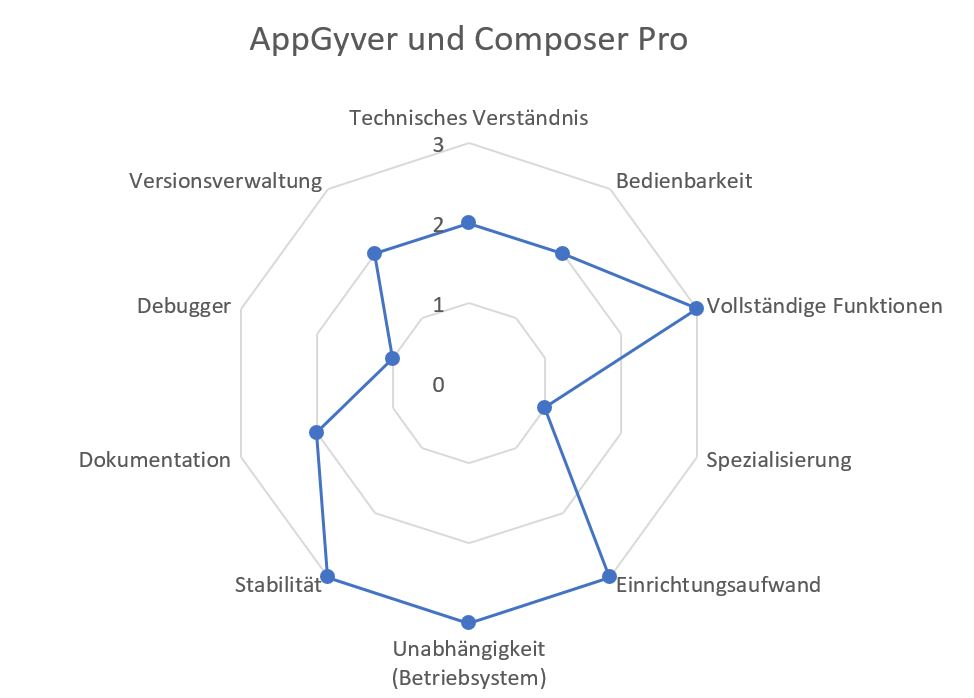
\includegraphics[width=0.7\textwidth]{Bilder/bewertung/ND_AppGyver_Comp.jpg}
 \caption{Bewertung von AppGyver Composer Pro }
\end{figure}
Er ist zwar für den Citizen Developer konzipiert, jedoch sind durch die komplexeren Konzepte auch grundlegende IT-Kenntnisse für die Bedienung des Composer Pro erforderlich. Die Schwächen der Entwicklungsumgebung fallen insbesondere im Vergleich zu Pro-Umgebungen auf: die rudimentäre Quellcode-Versionierung und die mangelhafte Debugger-Integration.

Die Vor-und Nachteile von AppGyver in Kombination mit Composer Pro:
\begin{table}[!htbp]
    \centering
     \setlength{\leftmargini}{0.4cm}
    \begin{tabular}{| m{6cm} | m{6cm} |}
        \hline
        \rowcolor{mygrey2} \makecell[c] {Vorteile} & \makecell[c] {Nachteile} \\
        \hline
         \begin{itemize} 
            \item Geringer Aufwand für die Implementierung der meisten Backend- und Frontendfunktionalitäten
            \item Flexibelität im App-Design
            \item Geringer Einrichtungsaufwand der Entwicklungsumgebung
            \item Unabhängigkeit der Entwicklungsumgebung von Betriebssystem 
            \item Stabilität von Composer Pro
        \end{itemize} & 
        \begin{itemize} 
            \item Wenig Ressourcen für Entwickler
            \item Spezifische Entwicklungsumgebung
            \item Debugger in Enterprise-Edition nicht verfügbar
            \item Quellcode-Versionierung in Community-Edition nicht verfügbar
        \end{itemize} \\
        \hline
      \end{tabular}
  \caption{Vor-und Nachteile von AppGyver mit Composer Pro} 
\end{table}

Aus den Vor- und Nachteilen kann folgendes Umsetzungsszenario abgeleitet werden:
\begin{itemize} 
  \item Durch die verfügbaren Funktionen, die flexible und schnelle Entwicklung, sowie die gute Integration von externen Services, lassen sich sehr viele Anwendungsszenarien umsetzen.
  \item Die Umsetzung kann dabei von einem Team aus reinen LCNC-Entwicklern erfolgen, ohne Zuarbeit von Pro-Entwicklern. Die Citizen Developer müssen jedoch über grundlegende IT- und spezielle AppGyver-Kenntnisse verfügen. 
\end{itemize}

\subsection{SAPUI5 in Verbindung mit SAPUI5}
SAPUI5 ist eine mächtige und sehr flexible Frontend-Technologie. Das Netzdiagramm zeigt, dass bis auf die Backend-Funktionalitäten alle untersuchten Frontend-Funktionalitäten in SAPUI5 umsetzbar sind. Allerdings  sind einige der Funktionalitäten mit hohem Programmieraufwand verbunden, wie z.B. die Pflegemaske eines einzelnen Produkts, die Nutzung mobiler Funktionalitäten und das Deployment für verschiedene Endgeräte.

SAPUI5 abstrahiert zwar bereits viel Logik in den Controls und es ist relativ einfach möglich, aus vielen Controls in einer View eine komplexere Anwendung zu erstellen, die Notwendigkeit die Ablauf-Logik aus zu programmieren (Events, etc.) ist jedoch ein Aufwandstreiber.
\begin{figure}[!htbp]
 \centering
 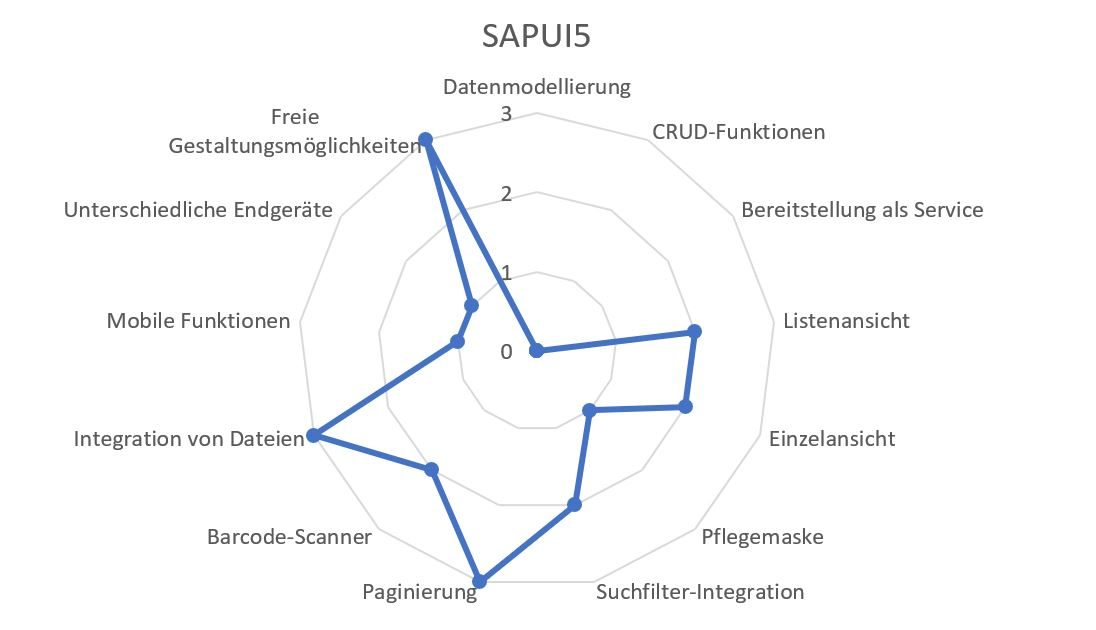
\includegraphics[width=0.7\textwidth]{Bilder/bewertung/ND_UI5.jpg}
 \caption{Bewertung von Umsetzung der Anforderungen in SAPUI5}
\end{figure}

Visual Studio Code ist eine offene Entwicklungsumgebung und es ist möglich, diese nach Belieben anzupassen. So sind auch alle notwendigen Funktionen für die SAPUI5-Entwicklung integrierbar und insbesondere die IT-Funktionalitäten sehr gut. 
\begin{figure}[!htbp]
 \centering
 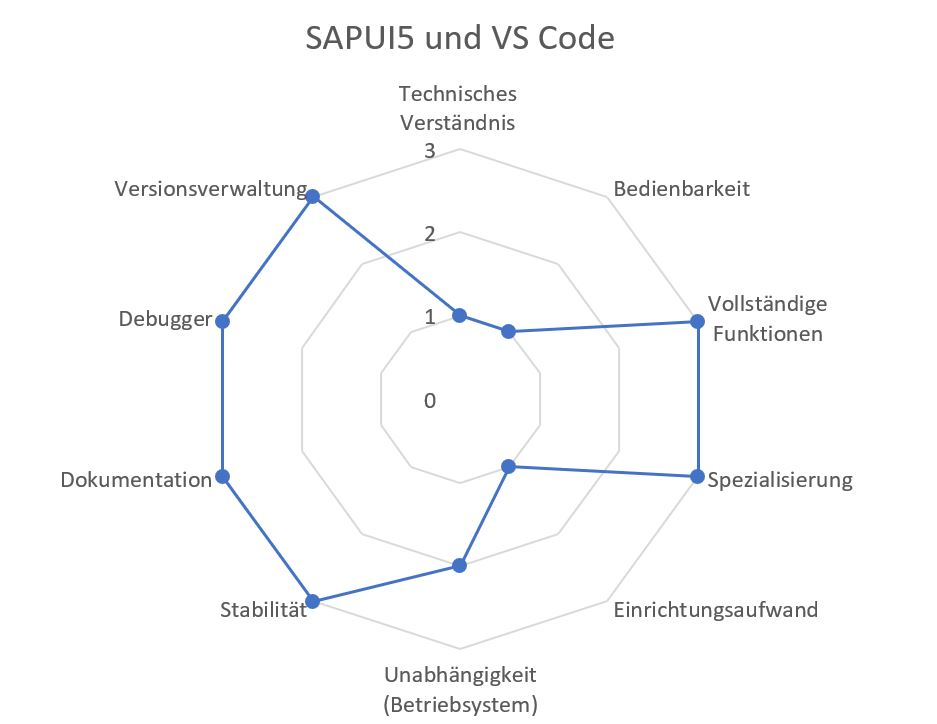
\includegraphics[width=0.6\textwidth]{Bilder/bewertung/ND_UI5_VSC.jpg}
 \caption{Bewertung von SAPUI5 mit VS-Code}
\end{figure}
Allerdings ist der Einrichtungsaufwand hoch und die Bedienung von VS-Code als klassische Programmierumgebung komplex. Daher ist SAPUI5 in Verbindung mit VS-Code nur für Pro-Code-Entwickler geeignet.


Die Vor- und Nachteile von SAPUI5 in Kombination mit VS-Code:
\begin{table}[!htbp]
    \centering
     \setlength{\leftmargini}{0.4cm}
    \begin{tabular}{| m{6cm} | m{6cm} |}
        \hline
        \rowcolor{mygrey2} \makecell[c] {Vorteile} & \makecell[c] {Nachteile} \\
        \hline
         \begin{itemize} 
            \item Sehr flexible Umsetzung möglich
            \item Weit verbreitete Entwicklungsumgebung
            \item Viele Hilfe-Ressourcen für Entwickler
            \item Sehr gute Entwicklungsumgebung mit fortgeschrittener Integration von Debugger-Funktionalitäten und und Versionsverwaltung Tools
        \end{itemize} & 
        \begin{itemize} 
            \item Großer Umsetzungsaufwand für verschiedene Funktionalitäten
            \item Großer Einrichtungsaufwand in VS Code
            \item Betriebssystem spezifische Entwicklungsumgebung
            \item Großer Lernaufwand für Anfänger
        \end{itemize} \\
        \hline
      \end{tabular}
  \caption{Vor- und Nachteile von SAPUI5 in Kombination mit VS-Code} 
\end{table}

Anhand der Vor- und Nachteile, sowie der diskutierten Details, lassen sich folgende Umsetzungsszenarien von SAPUI5 benennen:
\begin{itemize}
\item Entwicklung von komplexen Frontend-Applikationen, die von der Standard-Funktionalität (Fiori Element-Floorplans) abweichen in einem Team von Pro-Code-Entwicklern.
\end{itemize}